\documentclass[a4paper,11pt,twocolumn]{article}

\usepackage{icphs2023}
\usepackage{metalogo} % Only needed for the XeLaTeX logo
\usepackage{epstopdf}
%\usepackage{graphicx}


\graphicspath{{images/}}
\usepackage{subcaption}
%\usepackage[style=authoryear]{biblatex}
%\renewcommand*{\nameyeardelim}{\addcomma\addspace}

\usepackage{booktabs}
\usepackage[scale=2]{ccicons}

\usepackage{tipa}
\newcommand{\nt}[1]{\textipa{[#1]}} % narrow transcription
\newcommand{\wt}[1]{\textipa{/#1/}} % wide transcription

\hyphenpenalty=10000 % no hyphenation

\title{Coarticulation in Khalkha Mongolian harmonic and non-harmonic vowel sequences}
\author{XXX}
\organization{XXX}
\email{XXX}
\begin{document}

\maketitle

\begin{abstract}
In Khakha Mongolian, vowels in non-compound words share the features [ATR] and [round], with word-initial vowels triggering harmony in the carryover (left-to-right) direction. Vowel harmony has been variously understood as (i) emerging when listeners fail to perceptually compensate for acoustic variation due to coarticulation \cite{beddor2002}, or (ii) emerging for perceptual advantage in perceptually weak contrasts \cite{}. Towards understanding the relationship between these processes, this study quantifies coarticulatory variation in Khalkha Mongolian VCV sequences. We find that unlike harmonic sequences, non-harmonic sequences show greater propensity of coarticulation in the anticipatory (right-to-left) direction - opposite to that of vowel harmony. The high front vowel \wt{i}, which is transparent to harmony, also shows high coarticulatory resistance.
\end{abstract}

\keywords{Khalkha Mongolian, vowel harmony, coarticulation, vowels, acoustics}


\section{Coarticulation and Vowel harmony}



\section{Vowel system of Khalkha Mongolian}
     Seven phonological vowel categories, classified as non-pharyngeal (+ATR) and pharyngeal (-ATR) \cite{svantesson2005}: 

\begin{table}[!h]
	\small
	%\resizebox{\textwidth}{!} {%
		\begin{tabular}{@{}cccc@{}}
			\toprule 
			& [+ATR] & [-ATR]     & neutral                \\ \midrule
			high     & \textipa{u}                  & \textipa{U}    & \textipa{i} \\
			non-high & \textipa{e, o}               & \textipa{a}, \textipa{O} &                        \\ \bottomrule
		\end{tabular}%
		%}
	\caption{Monopthongs in Khalkha Mongolian, classified by harmony class}
	\label{table_vowels}
\end{table}     

\begin{itemize}
	\item Non-high vowels have rounded (right) and non-rounded (left) counterparts
	\item i : 2 allophones: \nt{i} in ATR words, \nt{I} in non-ATR words
\end{itemize}


\begin{itemize} 
	\item \textbf{Vowel harmony:} vowels in non-compound words must share the feature [ATR]. A subset of vowels (non-high: \textipa{e, o, a, O}) show rounding harmony.
	\item Focus of present study: ATR harmony
	\item \textbf{Directionality:} left-to-right
	\item \nt{i} is `transparent' $\rightarrow$ non-harmonic sequences
	
\end{itemize}


\subsection{Questions and Hypotheses}

\section{Materials and Methods}

\subsection{Materials}
We recorded 14 female native speakers reading 4 repetitions of 59 target words, in the frame [pi X gesen] ``I said X'' (critical items: 59$\times$14$\times$4 = 3304). Targets were disyllabic words of the form (C)V1CV2(C) \cite{svantesson2005}, and each vowel occurred in both initial (v1) and non-initial (V2) position. Words in which \wt{i} occupied the V2 position were classified as ``non-harmonic'', and all other words as ``harmonic''.

\subsection{Acoustic analysis}
A subset of recordings was used to train an acoustic model with the Montreal Forced Aligner \cite{mcauliffe2017montreal} to segment and annotate the data. We analyze Lobanov-normalized F1 and F2 at vowel midpoints. To quantify coarticulatory propensity, we use linear mixed effects models to examine how well the identity of V2 explains variance in the acoustics of V1 (anticipatory) and vice-versa (carryover).

\section{Results}
\subsection{Vowel space diffusion}

    \begin{figure}[!ht]
	\label{figure_combined}
	\centering
	\begin{subfigure}[t]{0.2\textwidth}
		\centering
		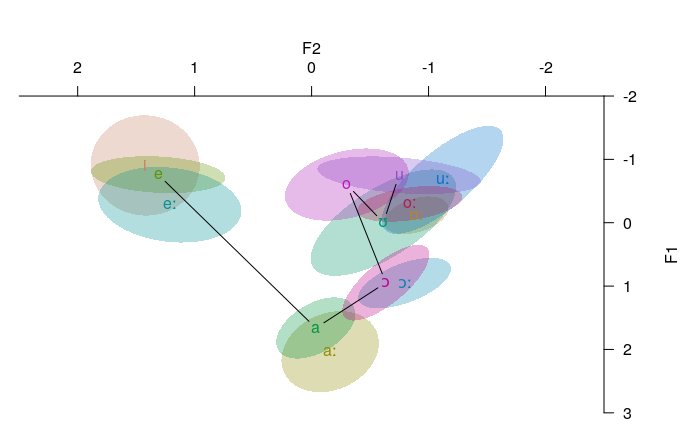
\includegraphics[scale=0.2]{har_v1.png} 
		\caption{harmonic subset: V$_1$} \label{har_v1}
	\end{subfigure}
	\begin{subfigure}[t]{0.2\textwidth}
		\centering
		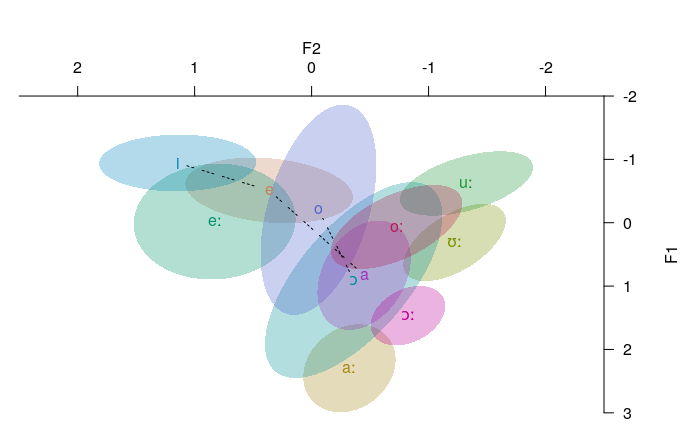
\includegraphics[scale=0.2]{har_v2.png} 
		\caption{harmonic subset: V$_2$} \label{har_v2}
	\end{subfigure}
	
	\begin{subfigure}[t]{0.2\textwidth}
		\centering
		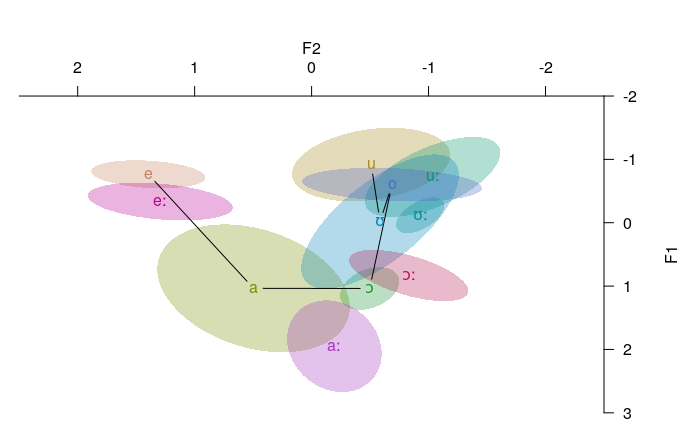
\includegraphics[scale=0.2]{nh_v1.png} 
		\caption{non-harmonic: V$_1$} \label{nh_v1}
	\end{subfigure}
	\begin{subfigure}[t]{0.2\textwidth}
		\centering
		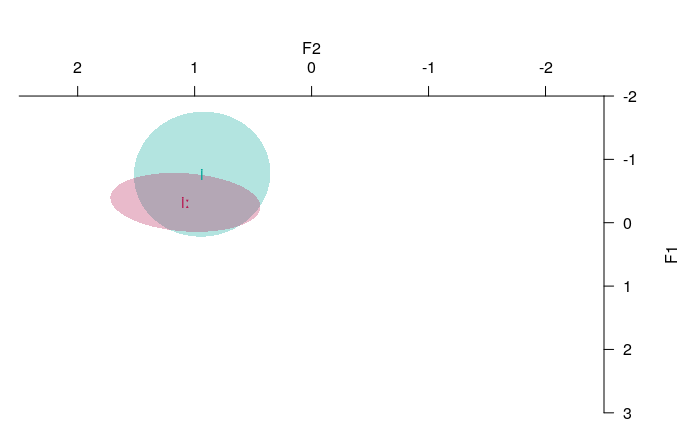
\includegraphics[scale=0.2]{nh_v2.png} 
		\caption{non-harmonic: V$_2$} \label{nh_v2}
	\end{subfigure}
	\caption{Steady-state formants for harmonic and non-harmonic vowel sequences}
\end{figure}

\subsection{Statistical analyses}

\subsubsection{F1}
Table \ref{table_results_f1} summarizes the final model and output for F1. Robust coarticulation in both directions, with greater propensity in the carryover (left-to-right) direction. 


\begin{table}[]
	%\small
	\resizebox{\textwidth}{!}{%
		\begin{tabular}{@{}lllllll@{}}
			\toprule
			Harmony type & Direction & Model fixed effects & ChiSq & Df & p & effect size ($\eta^2$) \footnote{using the effectsize package in R \cite{effectsize}} \\ \midrule
			\multirow{}{}{harmonic}     & anticipatory & F1V1t5 $\sim$ V1+\textbf{V2} & 17.174 & 9  & 0.04606 *     & 0.322 \\
			& carryover    & F1V2t5 $\sim$ V2+\textbf{V1} & 34.131 & 11 & 0.003443 *** & 0.536 \\ \midrule
			\multirow{}{}{non-harmonic} & anticipatory & F1V1t5 $\sim$ V1+\textbf{V2} & 100.87 & 1  & < 2.2e-16 *** & 0.133 \\
			& carryover    & F1V2t5 $\sim$ V2+\textbf{V1} & 133.41 & 10 & < 2.2e-16 *** & 0.174
		\end{tabular}%
	}
	\caption{Model outputs for coarticulation in F1, compared to a null model lacking the explanatory variable (bold)}
	\label{table_results_f1}
\end{table}


\subsubsection{F2}
Table \ref{table_results_f2} summarizes the final model and output for F2. Harmonic subset: coarticulation is left-to-right. Non-harmonic subset: greater anticipatory coarticulation (right-to-left)

\begin{table}[]
	%\small
	\resizebox{\textwidth}{!}{%
		\begin{tabular}{@{}lllllll@{}}
			\toprule
			Harmony type &
			Direction &
			Model fixed effects &
			ChiSq &
			Df &
			p &
			effect size ($\eta^2$) \\ \midrule
			\multirow{}{}{harmonic} & anticipatory & F2V1t5 $\sim$ V1+\textbf{V2} & 9.3863 & 9  & 0.4024        & 0.191 \\
			& carryover    & F2V2t5 $\sim$ V2+\textbf{V1} & 22.79  & 11 & 0.01892 *     & 0.404 \\ \midrule
			\multirow{}{}{non-harmonic} &
			anticipatory &
			F2V1t5 $\sim$ V1+\textbf{V2} &
			110.57 &
			1 &
			< 2.2e-16 *** &
			0.146 \\
			& carryover    & F2V2t5 $\sim$ V2+\textbf{V1} & 74.809 & 10 & 5.182e-12 *** & 0.101
		\end{tabular}%
	}
	\caption{Model outputs for coarticulation in F2, compared to a null model lacking the explanatory variable (bold)}
	\label{table_results_f2}
\end{table}	

\section{Discussion and Conclusion}

\bibliographystyle{IEEEtran}
\bibliography{references}

\theendnotes

\end{document}
